\documentclass[sigconf]{acmart}
% ===== Don't touch this :) ======
\settopmatter{printacmref=false} % Removes citation information below abstract
\renewcommand\footnotetextcopyrightpermission[1]{} % removes footnote with conference information in first column
\renewcommand\footnotetextauthorsaddresses[1]{}
\pagestyle{plain} % removes running headers
\graphicspath{ {./images/} }
% ================================
\usepackage{graphicx}
\usepackage{indentfirst}
\usepackage{float}
\usepackage{hyperref}
\usepackage{color}

\begin{document}
    \title{CS561 : Implementation of LSM-Tree}

    \author{Richard Andreas}
    \affiliation{%
        \institution{ra7296@bu.edu}
    }
    \author{Jingyu Su}
    \affiliation{%
        \institution{jingyusu@bu.edu}
    }
    \author{Xingkun Yin}
    \affiliation{%
        \institution{yinxingk@bu.edu}
    }

    \begin{abstract}
        In this paper, we explore the the design space of key-value stores that utilize the Log-Structured merge-tree (LSM-Tree) structure. More specifically, we have implemented a base version of the LSM-Tree that have been explored in previous work in order to get a better understanding of the basic knowledge of it. Instructions to compile and run the project are in the README.md of the repository of this project: \href{https://github.com/randreas/LSM_Tree_Repo}{\color{blue}{LSM Tree}}.
    \end{abstract}

    \maketitle

% =============================================================================
    \section{Introduction}
% =============================================================================

    \subsection{Motivation}


    Log-Structured merge-tree (LSM-trees) are one of the most commonly used data structures for persistent storage of key-value entries. LSM-tree based storages are in use in several modern key-value stores including RocksDB at
    Facebook, LevelDB and BigTable at Google, bLSM and cLSM at Yahoo!, Cassandra
    and HBase at Apache.


    \subsection{Problem Statement}
     In our paper, we will experiment on both Leveling and Tiering merging strategies with various workloads and compare their performance in 4 operations: insert, delete, point scan, range scan. We expect to discover a pattern on the performance differences between the two strategies, and answer the question.


% =============================================================================
    \section{Background}
% =============================================================================

    In this section, we will be presenting the background of LSM-trees, by discussing the basic structure of LSM-trees used in today's storage systems.

    \subsection{Basic Structure}
    Today's LSM-Tree implementation applies updates out-of-place to reduce Random I/Os. All incoming writes are appended into a memory buffer. An insert or update operation simply adds a new entry, while a delete operation adds a graveyard pointer indicating the entry has been deleted.

    A query over an LSM-Tree has to search multiple components to find the latest version of each key. A point look up query, which fetches the value of a specific key, simply search all components one by one, from newest to oldest, and stops immediately after the first match is found. A range scan can search all components at the same time, feeding the search results into a query.

    As components or data blocks accumulate over time, the query performance of an LSM-Tree tends to degrade since more components must be examined. These components are merged to reduce the total number of components. There are two types of merge policies, leveling and tiering. Both policies organize components or data blocks, into logical levels (or tiers) and controlled by a size ratio of T. Each component is labeled with its key range.

    In Leveling, each level only maintains one component, but the component at level L is T time larger than the component at level L-1. As a result, the component at level L will be merged multiple times with incoming components at level L-1 until it feels up, and it will then be merged into level L+1.

    In Tiering merge policy maintains up to T components per level. When level L is full, its T components are merged together into a new component at level L+1. If level L is already the configured maximum level, then the resulting component remains at level L. Two components at level L-1 are merged together to form a new component/data block at level L.\\
    \begin{figure}[H]
        \centering
        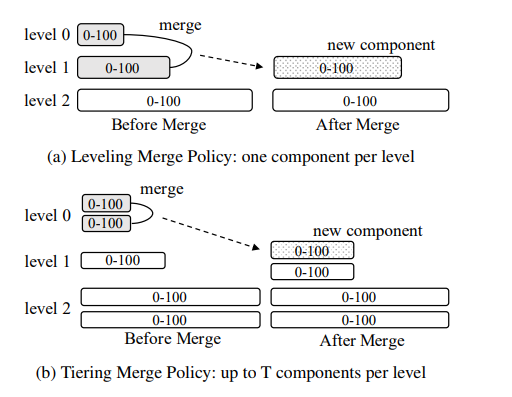
\includegraphics[width=0.5\textwidth]{MergingStrategies.PNG}
        \caption{LSM Tree merge policies}
        \label{Fig.main}
    \end{figure}
% =============================================================================
    \section{Architecture}
% =============================================================================
    \subsection{Components}
    In this section, we will analyze the main components of our LSM-Tree Architecture.
    \subsubsection{Tuple}
    Tuples are the units of data stored in a LSM-tree. In our implementation, a tuple consists of a key, a value that can contain multiple integers, and a tombstone indicator.
    \subsubsection{FileMeta}
    FileMeta corresponds to a block of data in a level. It is on persistent storage, in the case of this project, a local file. Filemata store the metadata of the block, including the path to the file, the size, the upper bound and the lower bounding of this file. When LSM Tree compact several blocks into one single block, the corresponding Filemetas are combined into a new Filemeta, and the new Filemeta contains all the metadata about the new block. The new Filemeta is then added to the next level.

    \subsubsection{Levels}
    Levels are the core in LSM trees as they contain actual data index. Our implementation of levels contain "FileMeta" objects, each of the FileMeta objects contain information necessary to access the correct data file on disk. Upon query, the LSM tree deserializes the data file with the information in the corresponding FileMeta, instantiates an Run object accordingly, and either return the result of query or modify the file. Run objects are destructed when query finishes.
    \subsubsection{Run}
    A run is the form of a materialized block of data in memory in a level of LSM tree. It contains the tuples sorted by key. Our level compaction operation involves reading all Filemeta of a level, create a run out of each of them, merge the runs into a big run, and create new data file and Filemeta accordingly.
    \subsubsection{Buffer}
    Operation log entries of the LSM tree goes directly into the buffer. Buffer in this project is an instance of Run. It has a fixed size, the same size as the blocks on the first level of the tree and it is the first data to look into when query. When the buffer if full, it is flushed into level 1, should level 1 be saturated, the compaction process of this LSM tree begins.
    \subsubsection{Bloom Filters}
    Bloom Filters are an essential component of the LSM-Tree that improves performance. The concept of a bloom filter is suggested as the main mechanism to avoid unnecessary level accesses. Queries first check the bloom filter, if the result is positive, then it checks the level, otherwise check a lower level or return not found if at bottom level. The main drawback is the possibility of giving a false positive result. When a level is compacted, it clears the corresponding bloom filter.
    \subsubsection{Fence Pointers}
    Fence Pointers are the limits of the virtual blocks of data. By implementing fence pointers, we are do not have to access every single data entry during scanning or point searching. We implement fence pointers in the form of zonemaps. By checking the min/max values in each fence pointer, and apply binary search in a data block with overlapping range, this reduces the time it takes for searching as we ignore blocks of data that do not meet the requirements.
    
    \subsection{Data File Organization}
    (This is preliminary implementation, may migrate into SSTable by final presentation).
    
    
    All data blocks besides buffer in our implementation are stored in binary files. Each block is stored in a file, and different blocks from different levels are differentiated by their filenames. For example, block 0 of level 1 will be named $level$-$0$-$block$-$0$.$bin$. Each file is organized as follows: 
    \begin{figure}[H]
        \centering
        \includegraphics[width=0.45\textwidth]{data_file.png}
        \caption{Data File Organization}
        \label{Fig.main1}
    \end{figure}
    The first SIZE$\_$OF$\_$INT bytes store the number of tuples in the file, 2 * SIZE$\_$OF$\_$INT * SIZE$\_$LIMIT number of bytes are reserved to store the start and end offset of each tuple, where SIZE$\_$LIMIT is the maximum number of tuples that can be stored in the data block, which is a parameter defined when the LSM tree is created. Each tuple start at its start offset storing its key with SIZE$\_$OF$\_$INT number of bytes, followed by its values. 
    
    When a tuple is to be added to the data block, which only happens in compaction of a leveling LSM tree, the tuple is appended directly to the end of the file, and only offsets are modified. 
    
    \subsection{Supported Operations/Features}
    The following are the operations our implementation supports, and some features it provides.
    \subsubsection{Insertion}
    Tuples inserted to LSM Tree goes directly into the buffer. When the buffer is full, it is flushed to the first level and persisted in a file described in the previous section, and appends a corresponding FileMeta object in the level. If a level is full, this triggers compaction.
    \subsubsection{Delete}
    Deletion is essentially a special type of insertion. A tuple with a special marker is inserted to the buffer, that indicates this tuple is a tombstone. Upon compaction, if the tombstone meets with a tuple with the same key, whichever is more up-to-date will live.
    \subsubsection{Range Delete}
    For range delete, we first do a range query to get all keys in the range that exists in the tree, then do deletion for each of them. (May eliminate the query process and do deletion of every key in range).
    \subsubsection{Point Query}
    For point query, we first do a binary search in the buffer, if the key isn't found, then we query the levels top-to-bottom. For each level, we first query the bloom filter, if it returns a positive, then go over the fence pointers to locate possible data blocks, then do a binary search on each data block for the result.
    \subsubsection{Range Query}
    The approach we take for range query is much like point query. When there is an overlapping data block, we do a linear scan to get tuples. A set of seen keys is maintained during the process to eliminate duplicates. 
    \subsubsection{Persistence}
    Our implementation supports persistence. When the LSM Tree is closed, it persists the data in the buffer in $buffer$.$bin$ in the same format as any other data block. It also stores the metadata in $metadata$.$bin$ so that when the LSM tree restarts, it can be reconstructed correctly. The metadata persisted includes: number of levels, buffer capability, size ratio between consecutive levels, the number of data blocks that currently resides in each level, and 1 byte for compaction policy. When the LSM tree restarts, it first read $metadata$.$bin$ for the coefficients, then reestablish buffer with $buffer$.$bin$, and finally levels and FileMeta.
    
    \subsubsection{Leveling/Tiering}
    User can choose compaction policy between leveling and tiering at the moment a LSM tree is first created. Once created the policy cannot be changed, because the metadata will be persisted, and the policy needs to stay consistent.
    

    \section{Testing}
    In order to correctness of our program, we have coded a simple program in python using hashsets on the same datasets and workload and outputs the same text file with operations as our project. By comparing both results, we ensure the correctness of the four operations in our prototype.

    In addition to correctness, we have tested our prototype with various sizes of data sets and workloads using both tiering and leveling merging strategies to compare the speed between both strategies on the same input files.
    
    \subsection{Experimentation Setup}
    
    We used the Microsoft Azure Virtual Machine to conduct our experiments. The configurations are as follows: Linux (Ubuntu 20.04) Operating System with Size: Standard B2s (2 vcpus, 4 GiB memory)
    
    \subsection{Benchmark Explanations}

    We used the data.wl and workload.wl files to test the correctness of our program. The data set covers the operation supported for now, and makes sure that the number of entries in the LSM tree is big enough to overflow the buffer, in order to trigger merge and tiering mechanism.


% =============================================================================
    \subsection{Results}
% =============================================================================
    Following are some graphs that provide some insights regarding the performance of our implementation. 

    \begin{figure}[H]
        \centering
        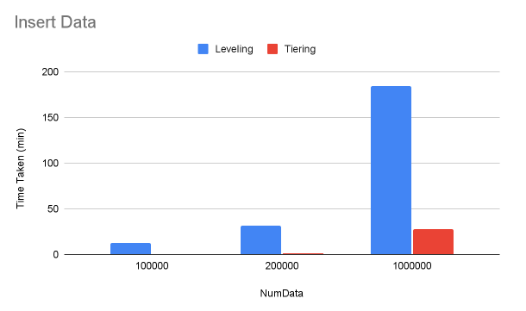
\includegraphics[width=0.45\textwidth]{LatencyInsert.PNG}
        \caption{Comparison between Tiering and Leveling for Insert}
        \label{Fig.main3}
    \end{figure}
    
    From our experiments, we can see that the time taken for data to be inserted using Tiering merge strategy is much faster than using the Leveling strategy as seen in Figure \ref{Fig.main3}. This solidifies the statement that Tiering as a merging strategy is more optimized towards write-heavy data compared to that of using Leveling.
    
    \begin{figure}[H]
        \centering
        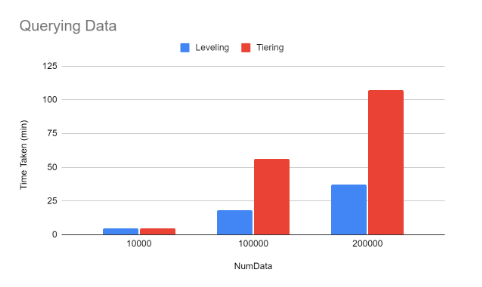
\includegraphics[width=0.45\textwidth]{LatencyQuery.PNG}
        \caption{Comparison between Tiering and Leveling for Read Heavy Workloads}
        \label{Fig.main4}
    \end{figure}
    
    Another experiment to compare tiering and leveling strategies on how they perform on read heavy workloads. In Figure \ref{Fig.main4}, we can see that the time taken for data to be inserted using Tiering merge strategy is much faster than using the Leveling strategy. This solidifies the statement that leveling as a merging strategy is more optimized towards read-heavy worloads compared to that of using tiering.

% =============================================================================
    \section{Future work to be done}
% =============================================================================

   The current implementation takes hours to process 1GB of data. We will need to do optimizations

% =============================================================================
    \section{Conclusion}
% =============================================================================
    
    LSM-Trees have become increasingly popular in modern NoSQL systems due to their advantages such as superior write performance, high space utilization and immutability of on-disk data and tunability. These factors have enabled LSM-trees to be widely adopted and deployed to serve a variety of workloads.
    
    In this paper, we have developed a prototype version of the LSM-Tree and have added some optimizations to improve the vanilla implementation. We hope that by implementing a LSM-tree from scratch, this will allow students to understand how it works, not just in theory but in practice as well.

% reference
        {
        \bibliographystyle{ACM-Reference-Format}
        \bibliography{biblio}

        [1] Chen Luo, Michael J. Carey. LSM-based storage techniques: a survey. VLDB J.29(1): 393-418 (2020)

        [2] Niv Dayan, Manos Athanassoulis, Stratos Idreos. Monkey: Optimal Navigable
        Key-Value Store. SIGMOD Conference 2017: 79-94

        [3] Patrick E. O'Neil, Edward Cheng, Dieter Gawlick, Elizabeth J. O'Neil. The LogStructured Merge-Tree (LSM-Tree). Acta Inf. 33(4): 351-385 (1996)
    }

\end{document}
